\chapter{Introdução} \label{Introducao}
%Contextualizar o problema e motivações
% Motivação (Por quê estes problemas/perguntas são relevantes?)

\section{Endereços e Geocodificação}

\epigraph{Quase tudo que acontece, acontece em algum lugar. Saber o local onde algo acontece pode ser fundamental.}{\cite{longley2013}}

No livro \cite{longley2013} os autores explicam a relação entre a humanidade e a localização. Para eles, é claro que a maior parte da atividade humana é feita no planeta Terra e por isso a vida é fortemente ligada a localidade. Sendo assim, entender e manipular informações geográficas está no cerne de qualquer aplicação que envolve a humanidade. Além disso, os autores explicam que decisões importantes podem causar consequências geográficas. Um exemplo seria uma movimentação financeira, que em um caso mais extremo, poderia causar uma crise econômica em uma determinada região.

No artigo \cite{Zamberg2009}, o autor traz aspectos importantes das informações geográficas que complementam o que foi dito anteriormente. Para ele, endereço é a principal forma de de conceitualizar localização no mundo atual. Isso se deve ao fato dos endereços serem utilizados em diversas aplicações de diferentes campos de estudo, como na saúde \cite{AmericaJournal2001,Kypri2009,Mazumdar2008}, nas ciências sociais \cite{Chow2011}, na análise de criminal ou judiciária \cite{Olligschlaeger1998}, na análise ambiental \cite{Gilboa2006}, na ciência da computação \cite{Zamberg2009}, na economia \cite{Whitsel2006} entre outras.

Para isso, é necessário gerar a representação computacional do endereço, de forma com que as aplicações possam utilizá-lo. A representaçãomais comum segundo \cite{Zamberg2009} é a representação por meio de coordenadas x e y em um plano, geralmente a medida é latitude e longitude. O processo de tranformação em um endereço nessas coordenadas é chamado de Geocodificação ou Georreferenciamento. Para \cite{Zamberg2009} esse processo consiste em 3 etapas:
\begin{itemize}
   \item Processamento do endereço de entrada: o endereço será lido, dividido em componentes (rua, número, bairro, etc), padronizado, cada campo é atribuído a uma categoria e por fim, serão indexadas as categorias necessárias; 
   \item Busca na base referência: de acordo com o algoritmo escolhido, será realizada uma busca na base referência afim de selecionar e classificar potenciais canditados para resposta;
   \item Seleção do(s) canditado(s) para resposta: com a busca realizada será feita uma análise da classificação gerada por ela e serão escolhidos os melhores canditados.
\end{itemize}

Segundo \cite{longley2013}, para além de representar computacionalmente um endereço, o georreferenciamento utilizando latitude e longitude tem diversas vantagens:
\begin{itemize}
   \item Sistema com precisão espacial: é capaz de indicar com precisão alta a localização de um certo endereço;
   \item Permitem cálculos de distância: por ser um sistema espacial, ele permeite que a distância e por consequência outras métricas sejam calculados para o endereço;
   \item Compreensão global: é um sistema utilizado mundialmente, sendo geralmente mais fácil de identificar e compreender; 
\end{itemize}

Apesar de todas as vantagens e aplicações, o processo de geocodificação pode causar informações erradas. No livro \cite{longley2013} os autores nomeiam essas falhas de informação como incertezas. Para coompreender o que é incertezas, é necessário levar em conta outros aspectos da falha na informação. Assim, são incluídos os conceitos:
\begin{itemize}
   \item Erro: Diferença entre o observado e o obtido;
   \item Falta de acurácia: Diferença entre a realidade e a nossa representação da realidade;
   \item Ambiguidade: mais de um valor igual ao outro;
   \item Indefinição: falta de informações necessárias. 
\end{itemize}

Após conceitualizar esses termos, eles definem incerteza como: ``medida da compreensão do usuário sobre a diferença entre o conteúdo de um conjunto de dados e os fenômenos reais que os dados devem representar'' \cite{longley2013}. A partir disso, incerteza foi aceita como uma boa medida de avaliação da qualidade dos Sistemas de Informação Geográfica (SIG). 

\begin{figure}[h]
   \centering
   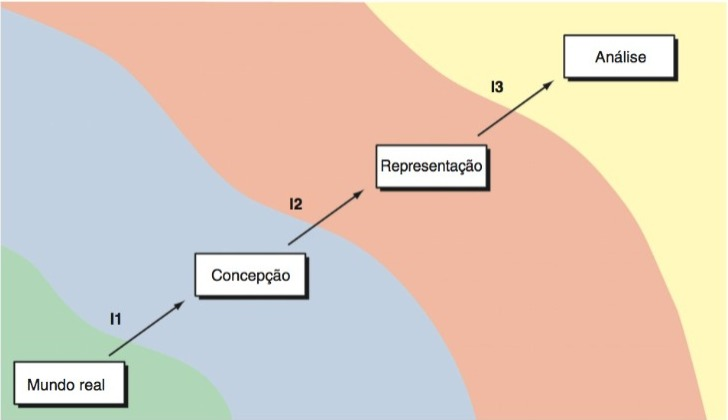
\includegraphics[width=\textwidth]{Figuras/incertezaLivro.jpeg}
   \caption{Retirada do livro \cite{longley2013}. Visão conceitual da incerteza, onde os filtros I1, I2, I3 distorcem a informação original}
   \label{fig:incerteza}
\end{figure}

\section{APIs de Geocodificação e Análise de qualidade}
% Revisão da literatura (O que já foi feito sobre o problema e o que falta fazer?)
% Definir o problema com precisão
   % Qual API erra mais?
   % Existe algum padrão espacial no erro?
   % Variância entre as APIs representa o erro?
\section{Objetivos}
% Objetivo (O que você pretente atingir?)
% Objetivos específicos (objetivos intermediários) 
O principal objetivo deste trabalho é avaliar o erro, a discrepância e a acurácia de cinco APIs utilizadas no laboratório de pesquisa e capacitação em desenvolvimento de software - TerraLAB. As APIs em análise são: Google Maps, TomTom, Open Route Service (ORS), Mapbox e Here. O erro será analisado quanto às respostas fornecidas pelas APIs diferirem do esperado. A discrepância medirá o nível de discordância entre as APIs. Por fim, a acurácia será utilizada para verificar a precisão das respostas fornecidas pelas APIs.

Uma parte essencial do trabalho é compreender os pontos onde essas APIs apresentam falhas, e, portanto, a análise espacial dessas medidas terá grande destaque na pesquisa.

Com isso, gostaríamos de responder as seguintes perguntas:
\begin{itemize}
   \item Qual API das utilizadas erra mais?
   \item Existe algum padrão espacial no erro?
   \item Alguma medida de variância entre as APIs (discrepância) representa o erro? 
\end{itemize}

Para chegar a essas  respostas temos alguns objetivos específicos que devem ser atendidos:
\begin{itemize}
   \item 
\end{itemize}





\section{Organização do Trabalho}

Um parágrafo fazendo uma descrição dos capítulos restantes do documento. 

\subsection{Estrutura da Monografia}

Segue uma \textbf{sugestão} para a estrutura da monografia: 

\begin{description}
   \item[Capítulo 1:] Introdução.
   \item[Capítulo \ref{RevisaoBibliografica}:] Revisão Bibliográfica/ Embasamento Teórico (com o referencial teórico e trabalhos relacionados).
   \item[Capítulo \ref{desenvolvimento}:] Metodologia ou Desenvolvimento (material e métodos).
   \item[Capítulo \ref{resultado}:] Resultados e Discussões.
   \item[Capítulo \ref{conclusao}:] Conclusão (e trabalhos futuros).
\end{description}


 









